%%%%%%%%%%%%%%%%%%%%%%%%%%%%%%%%%%%%%%%%%%%%%%%%%%%%%%%%%%%%%%%%%%%%%%%%%%%%%%%%%%%%%%%%%%%%%%%%%%%%%%%%%%%%%%%%%%%%%%%%%%%%%%%%%%%%%%%%%%%%%%%%%%%%%%%%%%%
% This is just an example/guide for you to refer to when producing your supplementary material for your Frontiers article.                                 %
%%%%%%%%%%%%%%%%%%%%%%%%%%%%%%%%%%%%%%%%%%%%%%%%%%%%%%%%%%%%%%%%%%%%%%%%%%%%%%%%%%%%%%%%%%%%%%%%%%%%%%%%%%%%%%%%%%%%%%%%%%%%%%%%%%%%%%%%%%%%%%%%%%%%%%%%%%%

%%% Version 2.5 Generated 2022/06/14 %%%
%%% You will need to have the following packages installed: datetime, fmtcount, etoolbox, fcprefix, which are normally inlcuded in WinEdt. %%%
%%% In http://www.ctan.org/ you can find the packages and how to install them, if necessary. %%%
%%%  NB logo1.jpg is required in the path in order to correctly compile front page header %%%

\documentclass[utf8]{frontiers_suppmat} % for all articles
\usepackage{url,hyperref,lineno,microtype,siunitx}
\usepackage[onehalfspacing]{setspace}



% Leave a blank line between paragraphs instead of using \\

\begin{document}
\onecolumn
\firstpage{1}

\title[Supplementary Material]{{\helveticaitalic{Supplementary Material}}}


\maketitle


\section{Methods}

\subsection{Additive STDP}
Equation \ref{eqs:methods:expAddSTDP} describes the STDP function used. The learning rate $A=\SI{0.2}{}$ was assigned so that the learning was slow. Recurrent weights were bounded $[0, 1]$.

\begin{equation}
    f(\tau) = 	\begin{cases}
                    A\text{ } \mathrm{exp} \left (%
                    \frac{-\tau}{\tau_{STDP}} \right ) & \mbox{if } \tau \geq 0 \\ \\
                    A\text{ } \mathrm{exp} \left (%
                    \frac{\tau}{\tau_{STDP}} \right ) & \mbox{if } \tau < 0
                \end{cases}
    \label{eqs:methods:expAddSTDP}
\end{equation}

\subsection{Multiplicative STDP}
Equations \ref{eqs:methods:expMulSTDP} and \ref{eqs:methods:expMulSTDP_half} describe the STDP function used where $w$ is the weight that is being updated. The learning rate $A=\SI{0.05}{}$ was assigned so that the learning was slow. Recurrent weights were bounded $[0, 1]$.

\begin{equation}
    f(\tau) = 	\begin{cases}
                    A\text{ } \mathrm{exp} \left (%
                    \frac{-\tau}{\tau_{STDP}} \right ) & \mbox{if } \tau \geq 0 \\ \\
                    A\text{ } \mathrm{exp} \left (%
                    \frac{\tau}{\tau_{STDP}} \right ) \text{ } w & \mbox{if } \tau < 0
                \end{cases}
    \label{eqs:methods:expMulSTDP}
\end{equation}

\begin{equation}
    f(\tau) = 	\begin{cases}
                    A\text{ } \mathrm{exp} \left (%
                    \frac{-\tau}{\tau_{STDP}} \right ) & \mbox{if } \tau \geq 0 \\ \\
                    A\text{ } \mathrm{exp} \left (%
                    \frac{\tau}{\tau_{STDP}} \right ) \text{ } \frac{w}{0.5} & \mbox{if } \tau < 0
                \end{cases}
    \label{eqs:methods:expMulSTDP_half}
\end{equation}

\section{Results}

When using additive STDP or multiplicative STDP (Eqs.~\ref{eqs:methods:expAddSTDP} and \ref{eqs:methods:expMulSTDP}/\ref{eqs:methods:expMulSTDP_half} respectively) activity increases and the weights converge to unimodal distributions, Fig.~\ref{supplementary:figs:results}. In the additive case, potentiation leads to increased activity, and increased activity leads to potentiation; this results in a unimodal distribution at the upper bound. In the multiplicative case, the distribution mean depends on the weight dependence: if weak, it is similar to additive, and if stronger, the weights converge to the weight dependence value. Under additive and multiplicative STDP, all neurons are recruited, and all fire at the maximum firing rate allowed under the refractory constraint.

%% Figures, tables, and images will be published under a Creative Commons CC-BY licence and permission must be obtained for use of copyrighted material from other sources (including re-published/adapted/modified/partial figures and images from the internet). It is the responsibility of the authors to acquire the licenses, to follow any citation instructions requested by third-party rights holders, and cover any supplementary charges.

%%% There is no need for adding the file termination, as long as you indicate where the file is saved. In the examples below the files (logo1.eps and logos.eps) are in the Frontiers LaTeX folder
%%% If using *.tif files convert them to .jpg or .png
%%%  NB logo1.eps is required in the path in order to correctly compile front page header %%%

\begin{subfigure}
\setcounter{figure}{1}
\setcounter{subfigure}{0}
    \centering
    \begin{minipage}[b]{0.32\textwidth}
        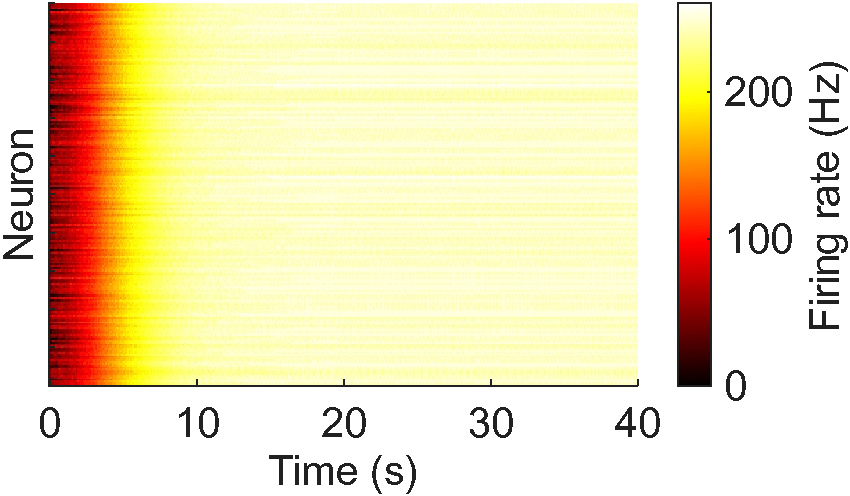
\includegraphics[width=\linewidth]{addSTDP/Hz.pdf}
        \caption{}
    \end{minipage}%   
\setcounter{figure}{1}
\setcounter{subfigure}{1}
    \begin{minipage}[b]{0.32\textwidth}
        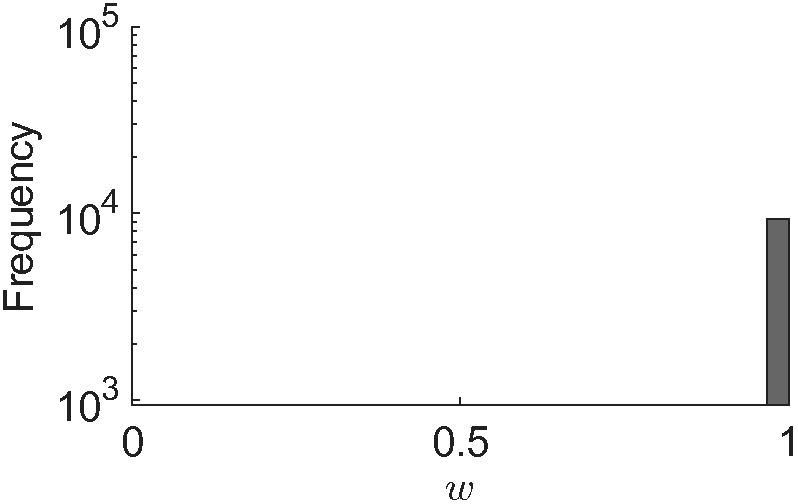
\includegraphics[width=\linewidth]{addSTDP/weights_E2E_histogram.pdf}
        \caption{}
    \end{minipage}%   
\setcounter{figure}{1}
\setcounter{subfigure}{2}
    \begin{minipage}[b]{0.32\textwidth}
        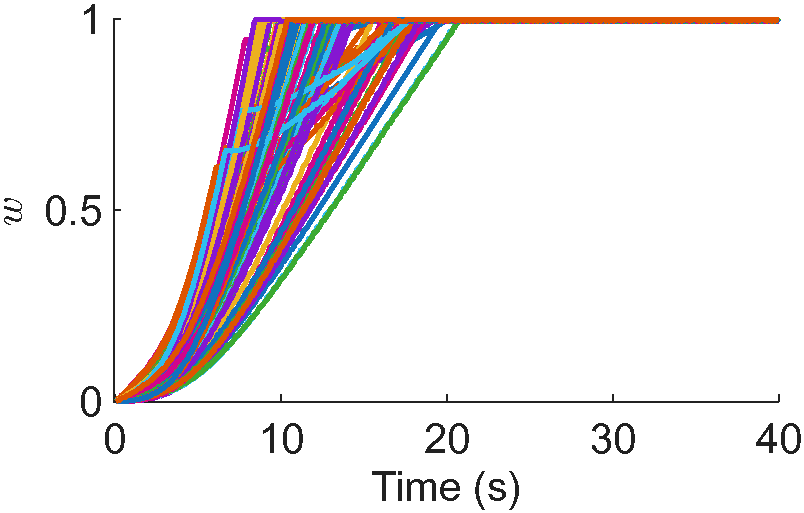
\includegraphics[width=\linewidth]{addSTDP/weights_E2E_traces.pdf}
        \caption{}
    \end{minipage}%   
\setcounter{figure}{1}
\setcounter{subfigure}{3}
    \begin{minipage}[b]{0.32\textwidth}
        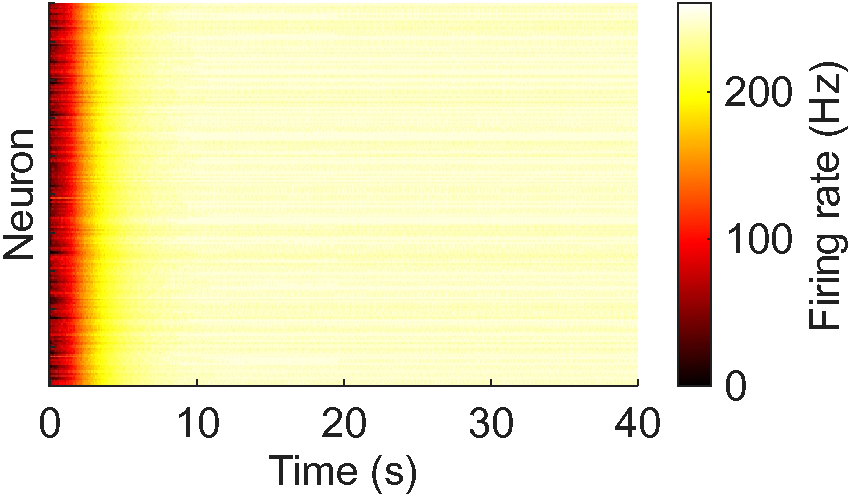
\includegraphics[width=\linewidth]{mulSTDP/Hz.pdf}
        \caption{}
    \end{minipage}%   
\setcounter{figure}{1}
\setcounter{subfigure}{4}
    \begin{minipage}[b]{0.32\textwidth}
        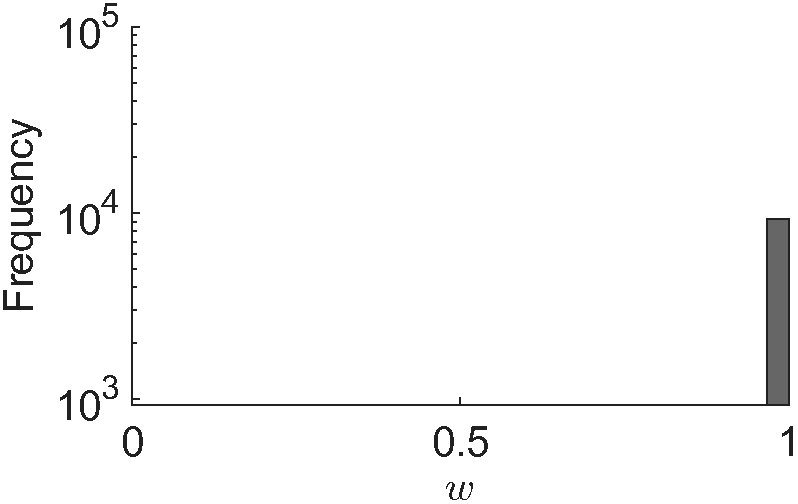
\includegraphics[width=\linewidth]{mulSTDP/weights_E2E_histogram.pdf}
        \caption{}
    \end{minipage}%   
\setcounter{figure}{1}
\setcounter{subfigure}{5}
    \begin{minipage}[b]{0.32\textwidth}
        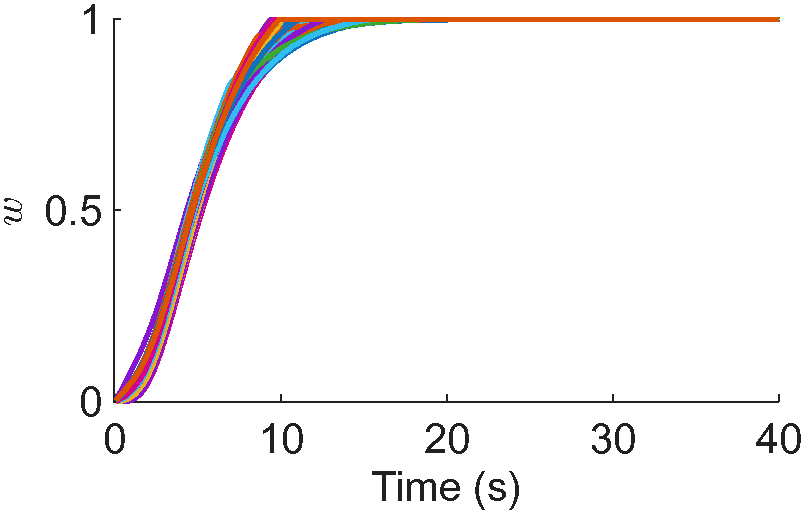
\includegraphics[width=\linewidth]{mulSTDP/weights_E2E_traces.pdf}
        \caption{}
    \end{minipage}
\setcounter{figure}{1}
\setcounter{subfigure}{6}
    \begin{minipage}[b]{0.32\textwidth}
        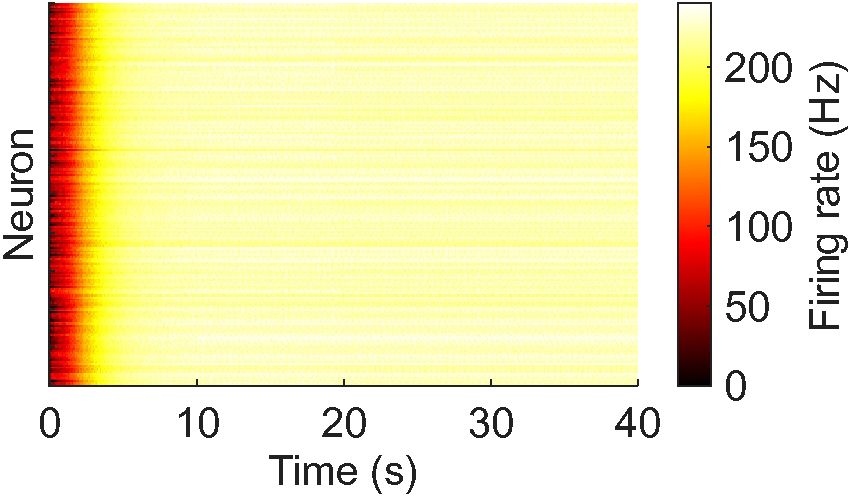
\includegraphics[width=\linewidth]{mulSTDP_half/Hz.pdf}
        \caption{}
    \end{minipage}%   
\setcounter{figure}{1}
\setcounter{subfigure}{7}
    \begin{minipage}[b]{0.32\textwidth}
        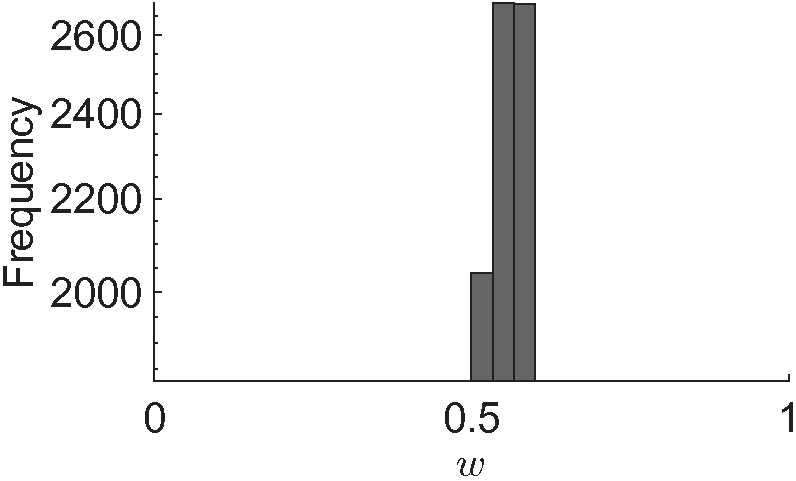
\includegraphics[width=\linewidth]{mulSTDP_half/weights_E2E_histogram.pdf}
        \caption{}
    \end{minipage}%   
\setcounter{figure}{1}
\setcounter{subfigure}{8}
    \begin{minipage}[b]{0.32\textwidth}
        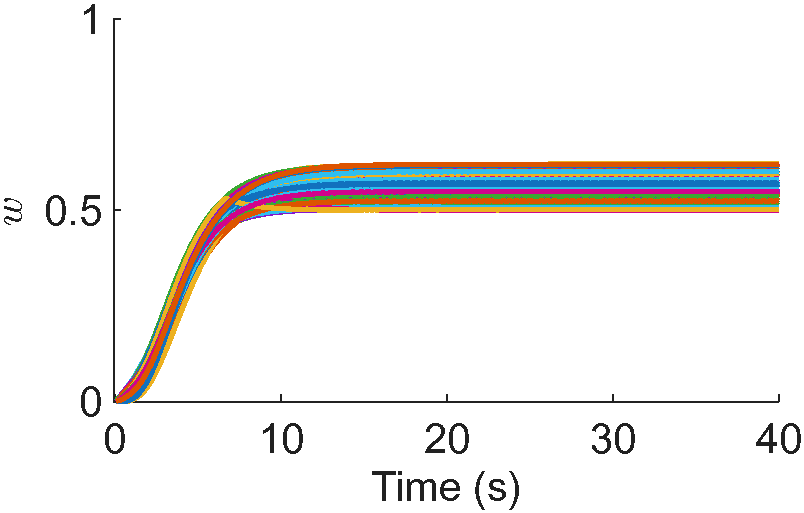
\includegraphics[width=\linewidth]{mulSTDP_half/weights_E2E_traces.pdf}
        \caption{}
    \end{minipage}

\setcounter{figure}{1}
\setcounter{subfigure}{-1}
    \caption{Typical network dynamics with additive or multiplicative STDP. \textbf{(A)} Firing rates of the network's neurons with additive STDP. \textbf{(B)} Weights, $w$, after learning with additive STDP. \textbf{(C)} Example of \SI{100}{} synapses' weights with additive STDP. \textbf{(D-F)} Same as A-C, but with multiplicative STDP with Eq.~\ref{eqs:methods:expMulSTDP} \textbf{(G-I)} Same as A-C, but with multiplicative STDP with Eq.~\ref{eqs:methods:expMulSTDP_half}}
    \label{supplementary:figs:results}
\end{subfigure}

%%% If you don't add the figures in the LaTeX files, please upload them when submitting the article.
%%% Frontiers will add the figures at the end of the provisional pdf automatically
%%% The use of LaTeX coding to draw Diagrams/Figures/Structures should be avoided. They should be external callouts including graphics.

\bibliographystyle{Frontiers-Harvard} %  Many Frontiers journals use the Harvard referencing system (Author-date), to find the style and resources for the journal you are submitting to: https://zendesk.frontiersin.org/hc/en-us/articles/360017860337-Frontiers-Reference-Styles-by-Journal. For Humanities and Social Sciences articles please include page numbers in the in-text citations 
%\bibliographystyle{Frontiers-Vancouver} % Many Frontiers journals use the numbered referencing system, to find the style and resources for the journal you are submitting to: https://zendesk.frontiersin.org/hc/en-us/articles/360017860337-Frontiers-Reference-Styles-by-Journal

% \bibliography{temp}

\end{document}
